
% File: template.tex
% InputFile: packages.tex
\documentclass[11pt,a4paper]{article}
\DeclareUnicodeCharacter{FB01}{fi}
	% Packages per la formattazione
	\usepackage{titlesec} % %package per le sezioni a quattro indici
	\usepackage[left=3.5cm,right=3.5cm,top=3.1cm,bottom=2.6cm]{geometry}
	\usepackage[italian]{babel}
	\usepackage[utf8]{inputenc}
	\usepackage{lastpage}
	\usepackage[T1]{fontenc}
	\usepackage{geometry}
	\usepackage{graphicx}%package per la gestione delle immagini
	\usepackage[font=small,labelfont=bf]{caption} %pakage per ridefinire font caption
	\usepackage{subcaption}  %package per le sottoimmagini
	\geometry{a4paper}
	\usepackage{fancyhdr} %package di style per  l/c/rhead l/rfoot
	\usepackage{tocloft} %package per i punti nella tableofcontents
	\usepackage{xr} %package per i riferimenti a label di file esterni
	\usepackage{longtable}
	\pagestyle{fancy}
	\usepackage{color} % sempre per i colori
	\usepackage[table]{xcolor} % package per i colori
	\usepackage{verbatim} %per scrivere codice e inserire commenti di più righe
	\definecolor{linkcolor}{cmyk}{1,.60,0,.40}
	\definecolor{acqua}{rgb}{0.0, 1.0, 1.0}
	\definecolor{blizzardblue}{rgb}{0.67, 0.9, 0.93}
	\definecolor{lightcyan}{rgb}{0.88, 1.0, 1.0}
	\definecolor{lightbrown}{rgb}{0.78, 0.7, 0.6}
	\definecolor{brown}{rgb}{0.65, 0.49, 0.32}
	\usepackage{hyperref}
		\hypersetup{
			colorlinks=true,
			linkcolor=black,
			urlcolor=linkcolor
		}		
	\usepackage{tabularx} %package meno complesso per la gestione delle tabelle
	\usepackage{svg} % package necessario per includere immagini .svg
	\usepackage{pdfpages}
	\usepackage{tikz} % package per disegnare figure
	\usepackage{eurosym} %package per il simbolo dell'euro
	\usepackage{multirow} %package per unire 2 righe
	\usepackage{pdflscape} %package per mettere il foglio in orizzontale (utile in caso di figure che si estendono in orizzontale)
	\usepackage{titlesec}
	\usepackage{listings}% package per riportare frammenti di codice 
	\usepackage{epstopdf}
% InputFile. commands.tex

%%INSERIRE IL NOME DEL DOCUMENTO
\newcommand{\documentName}{Relazione TecWeb}

%%INSERT THE CURRENT VERSION
\newcommand{\currentVersion}{1.0.0}

%%INSERT HERE DOCUMENT DATE
\newcommand{\redactionDate}{08/01/2020}

%%INSERT HERE THE NAME OF THE EDITORS
\newcommand{\editors}{
	\begin{itemize}
		\item Francesco Bari
	\end{itemize}
}

\newcommand{\verifiers}{\emph{Verificatore}}

%%DOCUMENT DISTRIBUTION LIST
\newcommand{\indirizzoweb}{\begin{itemize}
\item \url
\end{itemize}}

%%INSERIRE IL SOMMARIO
\newcommand{\informazioni}{Verbale interno con lo scopo di organizzare il lavoro all'interno del gruppo}


% BASE COMMANDS 
\newcommand{\email}{\textit{\href{mailto:francesco.bari.2@studenti.unipd.it}{francesco.bari.2@studenti.unipd.it}}}
\newcommand{\authorName}{\emph{cescomuch}}
\newcommand{\logo}{
\includegraphics[width=6cm,height=6cm]{../img/Unipd.pnh}}
\newcommand{\data}{\today}


\pagestyle{fancy}
\fancyhf{}
\setlength\headheight{26pt}
\rhead{ \documentName }
\lhead{
\includegraphics[scale=0.03]{../img/Unipd}}
\cfoot{\thepage}

% Linea nel footer 
\renewcommand{\footrulewidth}{0.4pt}

% 3 e 4 livello di profondita' per section e ToC
\setcounter{secnumdepth}{4}
\setcounter{tocdepth}{4}
\titleformat{\paragraph}
{\normalfont\normalsize\bfseries}{\theparagraph}{1em}{}
\titlespacing*{\paragraph}
{0pt}{3.25ex plus 1ex minus .2ex}{1.5ex plus .2ex}

% Indentazione prima linea dei paragrafi
\usepackage{indentfirst}




\begin{document}
	% <<<<< MODIFICARE
	\renewcommand{\documentName}{Relazione Tecnologie Web}								 
	\renewcommand{\currentVersion}{1.0.0}										 
	\renewcommand{\redactionDate}{08/01/2020}									 
	\renewcommand{\editors}{Francesco Bari\\ Ivan Furlan\\Francesco Pecile\\Lin Zhaohui \\}			
	
	\renewcommand{\verifiers}{admin@admin.com (\textbf{password:} admin) \\user@user.com (\textbf{password:} user) \\user2@user.com (\textbf{password:} user)}					
					
	\renewcommand{\informazioni}{\textbf{Indirizzo sito web:} \url{http://tecweb1920.studenti.math.unipd.it/ifurlan} \\ 
	\textbf{Email referente gruppo:} \email}



		
	% TITLE PAGE
       
	\begin{titlepage}
	\thispagestyle{empty}
	\setlength{\textfloatsep}{5pt}

	\begin{figure}[!t]
		\centering		
		
\includegraphics[width=6cm]{../img/Unipd} 
		\vspace{0.9cm}
	\end{figure}		
	
	\begin{center}	
			\vspace{1cm}
			\textcolor{black}{\textbf{\Huge\documentName}}
			\vspace{1cm}
			\begin{center}
				\textbf{\Large Informazioni sul documento} \\[0.5cm]
				\begin{center}	
				\begin{tabular}{ r | p{3.5cm} }
					\textbf{Nome documento} &  {\documentName}\\ \\
					\textbf{Versione} & {\currentVersion} \\ \\
					\textbf{Data redazione} & {\redactionDate} \\ \\
					\textbf{Membri} & \parbox{\textwidth}{\editors} \\ 
					\textbf{Users} & \parbox{\textwidth}{\verifiers} \\ 
				\end{tabular}
				\end{center}
			\vspace{0.5cm}
			\textbf{\Large Informazioni} \\[0.4cm]
			\informazioni
			\end{center}
	\end{center}
	\end{titlepage}
	
	\pagebreak
	


	\pagebreak
	\tableofcontents % indice
	\pagebreak
	\listoffigures
	\pagebreak
	
	% Contenuto del documento % <<<<< MODIFICARE
	%AGGIUNGERE QUA TUTTE LE SEZIONI
	\section{Introduzione}
\label{introduzione}

\subsection{Abstract}
Il progetto scelto dal gruppo ha come scopo la realizzazione di un sito dedicato ad un medico professionista di nome Marco Donati. Essendo un otorino, si specializza nei disturbi auditivi, posturali e nasali.

L’obiettivo della pagina è quello di far conoscere le capacità del dottore e metterlo in contatto con i propri pazienti.
Il sito web offre quindi quattro funzionalità principali:
\begin{itemize}
\item La possibilità di creare un account privato con il quale inviare messaggi privati tra l’utente e il dottore;
\item Una funzione di prenotazione visita online;
\item Le informazioni sulla locazione dello studio in cui saranno svolti i vari servizi medici disponibili e tutte le informazioni relative ad essi;
\item Una pagina nella quale verranno mostrate varie news, di tipo organizzativo piuttosto che informativo o di carattere divulgativo.
\end{itemize}

\subsection{Analisi d'utenza}
Il target del sito si concentra su uomini e donne di qualunque età in cerca di un consulto medico o di una prestazione medica specialistica.
Data l’ampiezza d’utenza potenzialmente molto variegata, il numero di utenti non avvezzi alla navigazione web potrebbe essere elevato, quindi si è deciso di sviluppare un design molto semplice ed efficace.
Le informazioni sono quindi fornite tramite l’utilizzo di un linguaggio informale e comprensibile, restando però nei limiti di comprensione imposti dal campo medico.
Il sito infatti mantiene comunque la professionalità e la precisione nei contenuti che si aspetterebbe un medico in visita nel sito.

Le informazioni fornite dal nostro sito sono di carattere puramente informativo, pensate per dare un’idea all’utente prima che incontri direttamente il dottore per spiegazioni molto più dettagliate.
Questa caratteristica fa sì che non sia necessaria una barra di ricerca, poiché la gran parte delle informazioni più complesse sarà data a voce o tramite il servizio di consulti online.
Si è pensato quindi di non doverla aggiungere in quanto l’espressività della barra di navigazione e delle sue sottosezioni copre completamente tutti i contenuti e le necessità dell’utente.

\subsection{Interazioni utente}

Abbiamo individuato 3 tipi di utente:
\begin{itemize}
\item Utente non registrato;
\item Utente registrato;
\item Admin.
\end{itemize}

L’utente non registrato può accedere a tutta la parte non interagibile del sito, ma può comunque informarsi su tutto il contenuto chiave senza doversi registrare.

L’utente registrato sblocca le funzionalità cardine del nostro servizio: la possibilità di prenotare un appuntamento tramite il nostro form online e consultare direttamente il dottore in modo privato.
Inoltre dopo aver prenotato una visita l’utente può visualizzarne privatamente le informazioni a riguardo ,così da poterle anche stampare per documentarsi.
Questa funzionalità è valida anche per tutte le conversazioni private con il dottore, le quali vengono mostrate tramite chat sullo schermo e possono essere eventualmente stampate.

L’admin del sito è lo stesso dottor Marco Donati, il quale ha poteri diversi dal semplice utente registrato, egli può:

\begin{itemize}
\item Aggiornare la pagina notizie, eliminando quelle vecchie e scrivendone di nuove;
\item Rispondere alle domande degli utenti registrati e visualizzare un elenco delle chat con tutti gli utenti;
\item Visualizzare una lista di tutte le prenotazioni delle visite, divise per giorno e tipologia.
\end{itemize}

Da notare il fatto che l’utente registrato e l’admin operano su due fronti ben diversi: l’admin non può modificare le prenotazioni fatte dall’utente se non in casi di emergenza dopo una notifica diretta paziente/dottore.
	\pagebreak
	\section{Organizzazione del lavoro e sviluppo}
\label{organizzazionelavoro}

\subsection{Progettazione}
Nella fase iniziale si sono individuate capacità e punti di forza dei membri del gruppo.
In seguito a ciò si è deciso di non affidare a ciascuno una parte ben precisa del progetto ma di svolgerlo nella sua interezza in gruppo, in modo da mantenere la coerenza del codice e delle idee su tutto il piano lavorativo.
Questa decisione inoltre garantisce che ogni membro del gruppo abbia lavorato su tutte le parti principali del progetto.
Abbiamo deciso di svolgere il lavoro in parallelo con le lezioni del corso, usando quindi una strategia di progettazione classica:
\begin{enumerate}
\item Codifica pagine HTML;
\item Codifica pagine CSS;
\item Creazione e popolamento Database;
\item Codifica JavaScript;
\item Codifica pagine PHP.
\end{enumerate}
Punto fondamentale degno di nota è l’accessibilità. Essa non è posta nell’indice della progettazione appena descritto, poiché sono stati fatti test continui ad ogni passo della progettazione.
Così facendo, ogni blocco di lavoro compiuto risulta accessibile e valido.
Questo ci ha consentito di non dover tornare sui nostri passi in fasi più avanzate del progetto, ma poter contare su una base di lavoro effettuato in modo costante.

Nello specifico sono state progettate le pagine dedicate alla due funzionalità più importanti del sito: la prenotazione della visita e il consulto online.
I punti cardine di queste due pagine sono:
\begin{itemize}
\item \textbf{Confidenzialità:} le informazioni relative alle prenotazioni e tutte le conversazioni tra dottore e utente possono essere accedute solo dai diretti interessati. Questa caratteristica è garantita dal fatto che l’accesso alle due pagine di prenotazione e consulti è consentito solo agli utenti registrati;

%AGGIUNGERE IMMAGINE PRENOTAZIONI

\item \textbf{Semplicità:} la pagina di consulti online utilizza un singolo form sul quale poter scrivere il proprio messaggio. Una volta fatto ciò la conversazione viene mostrata secondo i canoni standard della messaggistica online. La pagina prenota visita invece è composta da diversi form. In essi è possibile scegliere giorno, mese, anno e tipologia di prestazione. Controllando la disponibilità della data scelta sarà poi possibile visualizzare e quindi scegliere la fascia oraria libera più consona alle proprie esigenze orarie.

%AGGIUNGERE IMMAGINE CONSULTI ONLINE

\end{itemize}


\subsection{Design}
Abbiamo deciso di separare completamente la parte statica da quella dinamica, in modo da poter rendere semplice l’aggiornamento del sito in qualunque momento.
La struttura di ogni pagina web è templetizzata in modo
tale da incrementare robustezza del sito web, sul quale vengono applicati fogli di stile in CSS puri.
Tali layout in CSS sono stati sviluppati per ottenere un design fluido, scalabile e funzionale per la maggior parte dei browser e dei dispositivi.
Sul lato stilistico i colori scelti sono quelli standard che ci si aspetta da un sito web medico-sanitario. Comprendono infatti varie gradazioni di blu e bianco, le quali risultano rilassanti all’occhio.

\subsubsection{Header}
All’interno dell’header è presente il \textit{logo} del sito, i pulsanti \textit{accedi/registrati} e la \textit{navbar}.
Il \textit{logo} è situato a sinistra ed è caratterizzato da un link non circolare, ovvero funziona come link in tutte le pagine fatta eccezione per la home.
I pulsanti \textit{accedi/registrati} sono posti in alto a destra e dopo aver effettuato il login o la registrazione, spariscono, lasciando spazio ad un singolo pulsante \textit{esci} per uscire dal proprio account.
Infine la \textit{navbar} occupa una lunga linea che taglia tutto il sito orizzontalmente.
Questa ospita tutti i link alle pagine del sito ed è l’elemento centrale della navigazione nel sito web.
Bisogna notare che i link alle pagine non occupano tutta la lunghezza della navbar, ma sono posti il più possibile a sinistra.
Abbiamo scelto questo posizionamento perché, dagli studi fatti sul movimento oculare sugli utenti in una pagina web, si è ricavata una termografia dove le zone calde rappresentano le parti della pagina in cui l’utente ha dedicato più tempo, le quali risultano avere una forma ad F.
La disposizione dei nostri link fa uso di questa conoscenza per essere più accessibile dai nostri utenti. \\ \\

\begin{center}
\fbox{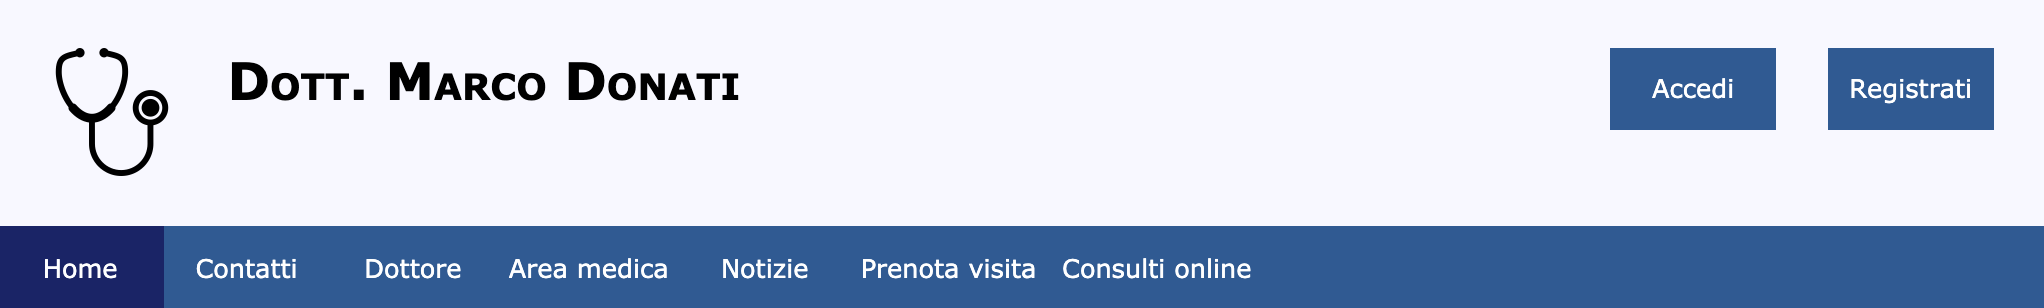
\includegraphics[width=12cm]{../img/header}}
\end{center}
\captionof{figure}{Header}


\subsubsection{Breadcrumbs}
Le \textit{breadcrumbs} sono presenti in tutte le pagine del sito, sia mobile che desktop, e comprendono un insieme di campi che identificano la posizione dell’utente all’interno del sito. L’ultimo campo è la pagina corrente, ovvero la pagina che l’utente sta visualizzando. Per evitare link circolari, quest’ultimo campo è solo testuale.

\begin{center}
\fbox{
\includegraphics[width=12cm]{../img/bread1}}
\end{center}
\captionof{figure}{Breadcrumbs utente non registrato}

\begin{center}
\fbox{
\includegraphics[width=12cm]{../img/bread2}}
\end{center}
\captionof{figure}{Breadcrumbs utente registrato}

\subsubsection{Contenuto}
Lo schema che abbiamo utilizzato è quello a tre panelli, i quali corrispondono alle seguenti domande:
\begin{enumerate}
\item \textbf{Dove mi trovo?} la prima risposta a questa domanda si trova nel titolo della pagina .La seconda si trova nelle \textit{breadcrumbs}, che indicano il percorso fatto per arrivare in quel punto;
\item \textbf{Di cosa parla questa pagina?} la risposta a questa domanda si trova nello stesso contenuto della pagina, diviso solitamente in due colonne, una posizionata a sinistra per seguire le regole date dalla termografia e una a destra contenente un immagine. Questa disposizione è dettata anche dal fatto che il contenuto delle pagine web si comporta in modo opposto a quello fisico. Ad esempio nei giornali le immagini prendono gran parte della pagina poiché attirano maggiormente l'attenzione, mentre nel web è il testo a fare da leader nell’attenzione ricevuta. Questo viene definito effetto zapping. Il nostro sito cerca di evitarlo;
\item \textbf{Dove posso andare?} la risposta a questa domanda si trova nella \textit{navbar} ,la quale non cambia mai di posizione. \\
\end{enumerate}

\begin{center}
\fbox{
\includegraphics[width=12cm]{../img/contenuto}}
\end{center}
\captionof{figure}{Esempio del contenuto di una pagina, in questo caso \textit{Notizie}} 

\bigskip

\textbf{Home} \\ 
Questa pagina ha la funzione di accogliere l’utente. È composta da uno \textit{slider} che mostra varie immagini del sito e da un testo che descrive il contenuto del sito sinteticamente.
Il testo è composto da meno di 100 parole, questo segue le regole base studiate da alcuni membri del gruppo durante il corso di WIM. Abbiamo quindi posto grande attenzione a restare nei limiti di tempo adeguati per mantenere l’attenzione degli utenti.
Infatti dopo vari studi è stato dimostrato che il tempo di permanenza in una pagina per il primo accesso da parte di un utente è 31 secondi; la nostra home in media rientra in questa tempistica. \\

\textbf{Pagina Contatti} \\ 
La funzione di questa pagina è di dare all’utente tutte le informazioni critiche su come contattare il dottore o trovare il suo studio medico.
Per fare ciò, oltre al testo contenente le varie informazioni, è stata inserita una mappa GoogleMaps interattiva. \\ \\

\textbf{Pagina Dottore} \\
Questa pagina serve ad introdurre la figura del Dott. Marco Donati, illustrandone le competenze e achievement professionali. \\

\textbf{Pagina Area Medica} \\
La pagina Area Medica racchiude tutte le 4 prestazioni mediche fornite dal dottore. Si compone quindi di 4 link alle pagine singole (nelle quali le prestazioni vengono spiegate nel dettaglio) e di brevi descrizioni per ciascuna di esse. \\

\textbf{Pagina Notizie} \\
La pagina Notizie raccoglie tutte le news postate dal dottore. È fondamentale per gli utenti poiché comprende informazioni piuttosto importanti circa le chiusure straordinarie dello studio medico, oltre a fornire documentazione su nuove terapie e funzionalità del sito in sviluppo. \\

\textbf{Pagina Prenota Visita} \\
Questa pagina viene divisa in 2 colonne. Entrambe ospitano dei form;
questi guidano l’utente registrato (gli utenti non registrati non possono accedere alla pagina) nella scelta di una data per una visita specialistica.
Si deve scegliere anno, mese, giorno, prestazione specialistica e quindi l’orario. \\

\textbf{Pagina Consulti Online} \\
Questa pagina è dedicata interamente alla chat privata con il Dottore.
Può essere acceduta solo da utenti registrati.
Per ogni messaggio inviato viene mostrato nome utente, data e orario di invio. \\

\textbf{Pagina Accedi} \\
Questa pagina viene utilizzata per accedere al sito del dottore previa registrazione. Per accedere bisogna inserire email e password. \\

\textbf{Pagina Registrati} \\
Questa pagina viene utilizzata per registrarsi al sito del dottore.  Per registrarsi è necessario fornire nome, cognome, numero di telefono, email e password. \\


\subsubsection{Footer}
All’interno del footer compaiono le immagini di validazione W3C HTML, W3C CSS, le informazioni relative al dottore (partita IVA, numero di iscrizione all’ordine dei medici) e i nomi degli sviluppatori. Le immagini per la validazione sono link cliccabili, che una volta premuti validano la pagina rispettivamente in xHTML 1.0 e CSS 3.

\begin{center}
\fbox{
\includegraphics[width=12cm]{../img/footer}}
\end{center}
\captionof{figure}{Footer}

\pagebreak

\subsubsection{Database}
Il nostro database è composto dalle tabelle:
\begin{enumerate}
\item \textbf{Messaggi:} contiene tutti i messaggi dei Consulti Online (sia degli utenti, sia del dottore);
\item \textbf{Notizie:} contiene tutte le notizie postate dal dottore;
\item \textbf{Utenti:} contiene tutti le informazioni legate agli utenti registrati;
\item \textbf{Visite:} contiene tutte le visite prenotate da utenti registrati.
\end{enumerate}

	\pagebreak
	\section{Implementazione lato front-end}
\label{frontend}

\subsection{HTML}
Si è deciso di usare xHTML 1.0 per garantire il supporto da tutti i tipi di web browser.
La parte di codifica in xHTML 1.0 ha posto le basi della struttura del sito ed è stata completata, nella sua interezza, come prima cosa.
Questa è stata templatizzata il più possibile per garantirne un riutilizzo efficace. Infatti sono stati creati in prima istanza l’header e il footer, così da poterli utilizzare in ogni pagina, e successivamente sono state creati ad hoc i contenuti di tutte le pagine.
Si è deciso di utilizzare HTML 5 per: 
\begin{itemize}
\item L’attributo \textit{placeholder} in tutti i form ove presente;
\item L’attributo \textit{maxlenght} in tutti i form ove presente;
\item L’attributo \textit{required} in tutti i form ove presente;
\item L’utilizzo della mappa interattiva Google Maps tramite il tag \textit{iframe}.
\end{itemize}

Strumento fondamentale per validare la correttezza del codice xHTML 1.0 e HTML 5 è stato il validatore fornito da W3C. Il validatore è stato settato con Document Type xHTML 1.0 Strict.
Da notare il fatto che le funzionalità HTML 5 sono state implementate per ultime, in maniera tale da preservare le funzionalità principali del sito nel caso in cui si utilizzi un browser che non supporta la suddetta versione di HTML. Questa caratteristica permette al nostro sito di “degradare elegantemente”.
\\
\\
Da menzionare il fatto che si è presa la decisione di definire il current link come classe e non come id, per evitare un conflitto con l’id delll’area medica precedentemente definito.

\subsection{CSS}
Fin da subito si è deciso di progettare 3 fogli di stile separati, rispettivamente: 
\begin{enumerate}
\item Stile desktop;
\item Stile mobile;
\item Stile stampa.
\end{enumerate}

\subsubsection{CSS desktop}
\label{frontend:css}
Scelte degne di nota sono state:
\begin{itemize}
\item Il logo, ritenuto molto importante in quanto associato dai clienti con lo studio, è stato inserito all’interno dell’HTML e poi modificato successivamente in CSS;
\item Tutte le immagini sono state adattate alla pagina usando il CSS.
\item Si è deciso di utilizzare una impostazione a due colonne per la maggior parte delle pagine;
\item Abbiamo differenziato l’uso di bold su CSS e strong/em in HTML, permettendo così il giusto funzionamento della lettura attraverso lo screen reader, sia la correttezza grafica del testo.
\item Per far si che con la riduzione della grandezza della pagina, le immagini del footer non occupino troppo spazio, abbiamo usato \textit{@media (max-width: 906px)}
\end{itemize}

\subsubsection{CSS mobile}
Le modifiche che abbiamo effettuato per l’adattamento alla versione mobile sono state:
\begin{itemize}
\item L’accesso/registrazione utente sono stati condensati in una singola icona, posta in alto a sinistra, la quale, se cliccata, mostra un piccolo menù a tendina che permette di scegliere se accedere o registrarsi;
\item Il menù di navigazione invece è stato implementato tramite un menù ad hamburger, il quale, al click, diventa un menù a tendina che occupa buona parte dello schermo ma senza nascondere completamente il contenuto della pagina;
\item Sono stati pensati 2 differenti punti di rottura:
\begin{enumerate}
\item Il primo a 630px orizzontali sancisce l’effettivo passaggio alla versione mobile;
\item Il secondo a 500px orizzontali prevede l’adattamento del logo e del titolo che vengono ridotti di circa il 50\%. In questo caso, anche il titolo che precedentemente non poteva essere cliccato, diventa cliccabile per sopperire alla poca superficie offerta dal logo rimpicciolito.
\end{enumerate}
\end{itemize}

\subsubsection{CSS stampa}
Il CSS  di stampa è stato scritto seguendo tutte le linee guida illustrate a lezione:
\begin{enumerate}
\item I link sono stati colorati in grigio (5e5e64) (per garantire una stampa full b/w) e l’indirizzo URL è stato esplicitato;
\item Le breadcrumbs sono state rimosse;
\item Il menù di navigazione è stato rimosso;
\item La mappa di Google Maps è stata rimossa dalla stampa, poichè non è ritenuta utile in quanto immagine statica;
\item La disposizione dei form della pagina prenota visita è stata cambiata per esser visualizzata meglio su carta;
\item In alto, accanto alla data, è stata lasciata la stampa dell’id pagina (esempio Consulti Online-Dott Marco Donati per la pagina consultionline.html) per dare più contesto;
\item L'id del logo è stato definito sull'ancora piuttosto che sull'immagine affinché nel CSS di stampa, alla richiesta di mostrare l’indirizzo web dei link, l’indirizzo del logo non venga mostrato.
\end{enumerate}

\subsection{Compatibilità con browser datati}
Per garantire la compatibiltà con browser datati:
\begin{itemize}
\item All’interno dei form sono stati usati \textit{type text} per le email e il \textit{type number} per i numeri telefonici, scegliendo quindi di non utilizzare \textit{type email} e \textit{type tel};
\item \textit{sticky} viene messa in coda al codice come tutte le altre funzioni CSS3,  così che, se la pagina venisse aperta da un browser che non supporta CSS3 la funzionalità della pagina non verrebbe compromessa, semplicemente le funzioni CSS3 opzionali non sarebbero mostrate. Questo vale anche per proprietà come \textit{border-radius}, \textit{box-sizing};
\item Non usando CSS3 non è possibile fare radio button colorati, quindi un user di IE8 o precedenti vedrà solo dei pallini senza colore. Questo però non inficerà sulla usabilità perché i radio button cliccabili saranno comunque distingubili da quelli non cliccabili;
\item Come detto in precedenza §\ref{frontend:css} abbiamo usato \textit{@media flex}, questa usa CSS3 ma pur non essendo supportata non degrada in modo particolare il sito. Anzi è solo una questione puramente estetica;
\item Per quanto riguarda la mappa di Google Maps, per utilizzarne la funzionalità  non abbiamo avuto scelta se non usare funzioni HTML 5, che quindi risultano errate in un validatore xHTML 1.0 Strict. (Come è stato detto a lezione);
Quindi nella pagina contatti, il documento è stato dichiarato come HTML 5, unica eccezione del nostro sito.
\end{itemize}


	\pagebreak
	\section{Accesibiltà}

Il sito mantiene la completa separazione tra struttura, presentazione e comportamento. La struttura è stata sviluppata tramite documenti xHTML, i quali richiamano i fogli di stile esterni CSS puri che implementano la presentazione, ed infine, per quanto riguarda il comportamento, sia script esterni realizzati con JavaScript che pagine dinamiche in PHP.
Tutto il codice redatto è stato scritto secondo le raccomandazioni W3C WCAG 2.0 (Level AAA).
Si sono evitati tag e attributi deprecati. \\

\subsection{Screen reader}
Sono stati effettuati vari test tramite screen reader, cercando il più possibile di simulare l’esperienza di un non vedente sul nostro sito. Così facendo sono state individuate le criticità e sono state quindi sviluppate tecniche per risolverle. \\


La criticità più fastidiosa era data dalla mancanza di \textit{skipLink} efficaci;
sono quindi stati introdotti 3 diversi \textit{skipLink}:
\begin{itemize}
\item Il primo è posto all’inizio della pagina e fa saltare il logo andando al contenuto principale della pagina stessa;
\item Il secondo è presente solo nella pagina contatti e permette di saltare la mappa di Google Maps;
\item Il terzo è posto poco prima del footer e riporta l’utente alla barra di navigazione. Si è pensato infatti che l’utente, dopo aver visitato l’intera pagina, voglia poterne visitare un’altra e viene quindi ridirezionato al menù di navigazione stesso. \\ 
\end{itemize}



Lo \textit{slideshow} è stato programmato in modo da non creare fastidi ai non vedenti. A tal proposito è stato illuminante il seminario svolto in classe.
Il nostro \textit{slideshow} infatti non reagisce con lo screen reader, poiché non cambia in automatico le immagini. Viene inoltre data la possibilità di saltarlo direttamente tramite \textit{skipLink.}\\

Le parole in lingue diverse da quella italiana sono state racchiuse all'interno di tag con l'attributo \textit{lang}, per permettere una corretta lettura da parte dello screen reader.\\


Abbiamo infine provato a navigare i form senza l’uso del mouse e siamo rimasti soddisfatti dal risultato dopo aver corretto vari errori nell’HTML.
I \textit{radio button} che normalmente sono colorati di verde se un’ora è disponibile o di rosso se invece non lo è (totalmente inutile in caso di cecità) sono stati modificati facendo in modo che al passaggio sul form, il pulsante dichiari il suo stato di disabled o meno.\\

\subsection{Colori}

I colori, a tema medico, sono stati scelti in modo da seguire le regole del contrasto e raggiungono un livello di accettabilità tripla A. (In particolare, ratio 7.14:1 tra \#2E5894 e \#FFFFFF, e di 14.39:1 tra \#192168 e \#FFFFFF).
Questi inoltre restano ben distinti anche usando una scala di grigi o con alterazione/mancanza di colori.\\

\subsection{Test}

Tutti i test riguardanti l’accessibilità sono stati svolti (e passati) con:
\begin{itemize}
\item \textit{Total Validator;}
\item \textit{Silktide Screen Reader Simulator;}
\item \textit{Color Contrast Analyzer};
\item \textit{Wawe.}
\end{itemize}

I feedback dati da questi test ci hanno quindi permesso di redarre le sezioni riguardanti l'accessibilità.


	\pagebreak
	\section{Implementazione lato back-end}

\subsection{PHP}
Il comportamento del sito dal lato server è gestito da file PHP, i quali sostituiscono completamente i controlli JavaScript nell'eventualità che sia disabilitato o non disponibile. I file PHP interagiscono con il database, forniscono sessioni di utilizzo per utenti loggati (incluso l'admin) e caratterizzano il comportamento generale delle pagine. Le funzioni più utilizzate e generali sono state definite in un file a parte \textit{funzioni.php}, mentre i file specifici per ogni pagina contengono le funzioni di utilità a loro associati. 

Descriviamo quindi le funzioni di maggiore importanza contenute in \textit{funzioni.php}:
\begin{itemize}
\item \textbf{getPaginaHTML(pageName)}: Funzione che, ricevuto in ingresso la pagina corrente, ne recupera il file HTML corrispondente e successivamente:
\begin{itemize}
\item ci inserisce Header e Footer;
\item mostra il pulsante Esci se si è loggati;
\item inserisce i breadcrumbs
\item nel casi si sia admin modifica le voci del menu di navigazione "Prenota visita" e "Consulti online" rispettivamente in "Visite prenotate" e "Elenco chat"
\item elimina i link ricorsivi.
\end{itemize}
Una volta eseguiti questi passaggi ritorna una stringa contenente la pagina HTML, senza eventuale contenuto dinamico all'interno del main (che sarà da gestire poi nella relativa pagina).
\item \textbf{controlloCampiDatiRegistrati(nome, cognome, telefono, email, password, confermapassword)}: Funzione che, ricevute in ingresso le credenziali del form di registrazione, ritorna true se e solo se tutti i dati sono stati compilati correttamente (non vuoti e conformi alle espressioni regolari a loro corrispondenti), altrimenti ritorna una stringa contenente gli errori relativi ai campi compilati erroneamente;
\item \textbf{preparaHTMLListaVisite(arrayVisite)}: Funzione che riceve un array dove ogni elemento è a sua volta un array con le informazioni della singola visita. Ritorna una stringa contenente la lista delle visite in codice HTML.\\
\end{itemize}


Descriviamo inoltre le funzioni degne di nota relative alla connessione con il database contenute in \textit{dbaccess.php}:
\begin{itemize}
\item \textbf{\_\_destruct()}: ridefinisce il distruttore della classe, in modo che chiuda la sessione corrente con il database (qualora sia stata aperta);
\item \textbf{openDBConnection()}: apre la connessione con il database;
\item \textbf{login(email, password)}: se il login avviene con successo ritorna l'email, nome e cognome dell'utente, altrimenti ritorna false;
\item \textbf{registrazioneUtente(email, nome, cognome, telefono, password)}: ritorna true se la registrazione è andata a buon fine, altrimenti ritorna false;
\item \textbf{getListaVisitePrenotatePeriodo(periodo, email, getNomeUtente)}: questa funzione ritorna un array con le visite prenotate in un determinato periodo che viene passato come parametro. Questo parametro è una stringa contenente un codice per identificare il periodo desiderato (E. "f7" indica i prossimi 7 giorni da oggi, "20p" indica le ultime 20 visite già passate) \\I parametri email e getNomeUtente sono opzionali, infatti se non viene passato il campo email vengono considerate le visite di qualsiasi account, mentre getNomeUtente, che serve per dichiarare se si vuole ricevere anche i dati relativi a chi ha prenotato la visita, di default è true.
\end{itemize}

\pagebreak

Infine, descriviamo le scelte implementative degne di nota relative alle singole pagine: \\

\textbf{registrati.php} \\ 
Nel contesto dell'inserimento errato delle credenziali, la pagina, una volta ricevute tramite form le informazioni da inviare al database, notifica gli errori relativi all'inserimento dei campi errati, mantenendo però le informazioni corrette precedentemente inserite dall'utente. Questo per evitare all'utente di dover reinserire nuovamente tutte le informazioni. \\ \\

\textbf{accedi.php} \\ 
Per quanto riguarda questa pagina, la funzionalità descritta nel paragrafo precedente non è stata implementata. Questo per non dare troppe informazioni ad un eventuale utente malevolo, relativo al campo immesso erroneamente. Infatti, se mostrassimo quale campo si è sbagliato, lasciando inserito quello corretto, daremmo delle informazioni che potrebbero essere usate in modo malintenzionato. \\ \\

\textbf{controllaDisponibila.php} \\
Questa pagina serve solo per stampare un file in formato JSON che viene utilizzato come API da JavaScript in \textit{prenotavisita.php}. Se non dovessero esserci variabili impostate, si viene reindirizzati alla pagina 404 (per esempio se si dovesse provare ad accedere alla pagina copiando un URL).
Non serve controllare che la data sia corretta, perché questa pagina viene chiamata soltanto da JavaScript, che quindi dovrà essere attivo (e deve aver già fatto i controlli).
Se JavaScript non dovesse essere attivo i controlli saranno semplicemente fatti lato server tramite PHP quando verrà inviata la richiesta, e quindi questa pagina non verrà chiamata. \\ \\

\textbf{prenotavisita.php} \& \textbf{consultionline.php} \\
Se non si è loggati, il sito lo riconosce e invita il visitatore ad effettuare l'accesso oppure a compiere la registrazione. Tutto questo è stato implementato tramite PHP. \\ \\

\textbf{notizie.php} \\
Il form relativo all'inserimento e alla modifica di una notizia è lo stesso, cambia solo il valore del pulsante \textit{submit}, che poi (sempre in PHP) serve ad identificare l'azione corrispondente. \\ \\

\bigskip
\bigskip

Una ultima precisazione in merito alle pagine contenenti form: è presente un tag \textit{<erroriDaMostrare />} che, nel caso ci siano errori, viene sostituito con gli errori che devono essere mostrati  relativi alla singola pagina, mentre se non ce ne sono viene semplicemente sostituito dalla stringa vuota.








	\pagebreak
	\section{Ruoli}

Di seguito si elencano le parti alle quali hanno contribuito i membri del gruppo:

\begin{itemize}
\item \textbf{Francesco Pecile}
\begin{enumerate}
\item HTML di alcune pagine;
\item CSS di alcune parti del sito;
\item Alcune funzioni JavaScript;
\item Test di accessibilità;
\item Stesura relazione.
\end{enumerate}

\item \textbf{Francesco Bari}
\begin{enumerate}
\item HTML di alcune pagine;
\item CSS di alcune parti del sito;
\item Alcune funzioni JavaScript;
\item PHP di alcune pagine;
\item Stesura relazione.
\end{enumerate}

\item \textbf{Ivan Furlan}
\begin{enumerate}
\item HTML di alcune pagine;
\item CSS di alcune parti del sito;
\item Alcune funzioni JavaScript;
\item PHP delle pagine;
\item Contributo informazioni relazione.
\end{enumerate}

\item \textbf{Lin Zhaohui}
\begin{enumerate}
\item HTML di alcune pagine;
\item CSS di alcune parti del sito;
\item Funzioni JavaScript;
\item PHP di alcune pagine;
\item Contributo informazioni relazione.
\end{enumerate}
\end{itemize}
	\pagebreak
	
\end{document}
